\chapter{Basics}
%\textcolor{red}{
%Everything necessary to understand the implementation as well as anything which is done beforehand, will come up here}

In this chapter, all concepts, technologies and required backgrounds for understanding this thesis, as well as the showcase implementation, are explained. First data and data types are described, second diagrams and how they are structured are described. Last D3 as the tool to create diagrams is described and its core concepts explained.


\section{Data}
%\textcolor{red}{
%Well talk about data a bit. Where does it come from? How is it structured? What kind of attributes? What even are attributes?}

Since ancient times, humans have recorded data. Recording the ins and outs of available resources and other administrative record-keeping were one of the driving factors behind the conceptualization of writing\cite{senner1991origins}.
With the introduction of computers the amounts of gathered data have grown drastically. Nowadays vast amounts of data are gathered across all aspects of life. The total amount of data created, consumed and stored by 2020 was already at 64.2 zettabytes and is projected to reach about 180 zettabytes by 2025\cite{statista_2022}.

The vast amounts of data gathered in databases are often hard to comprehend and evaluate with the human mind. They are also unwieldy to present them in the often limited space of articles, dashboards or other informative purposes. Therefore data visualization (Figure \ref{fig:data-visualization}) is used to turn these datasets, which are collections of data-points, into diagrams. These diagrams can easily be shown in more limited spaces, as well as allow for a quick general understanding and overview of the provided data.

\begin{figure}
    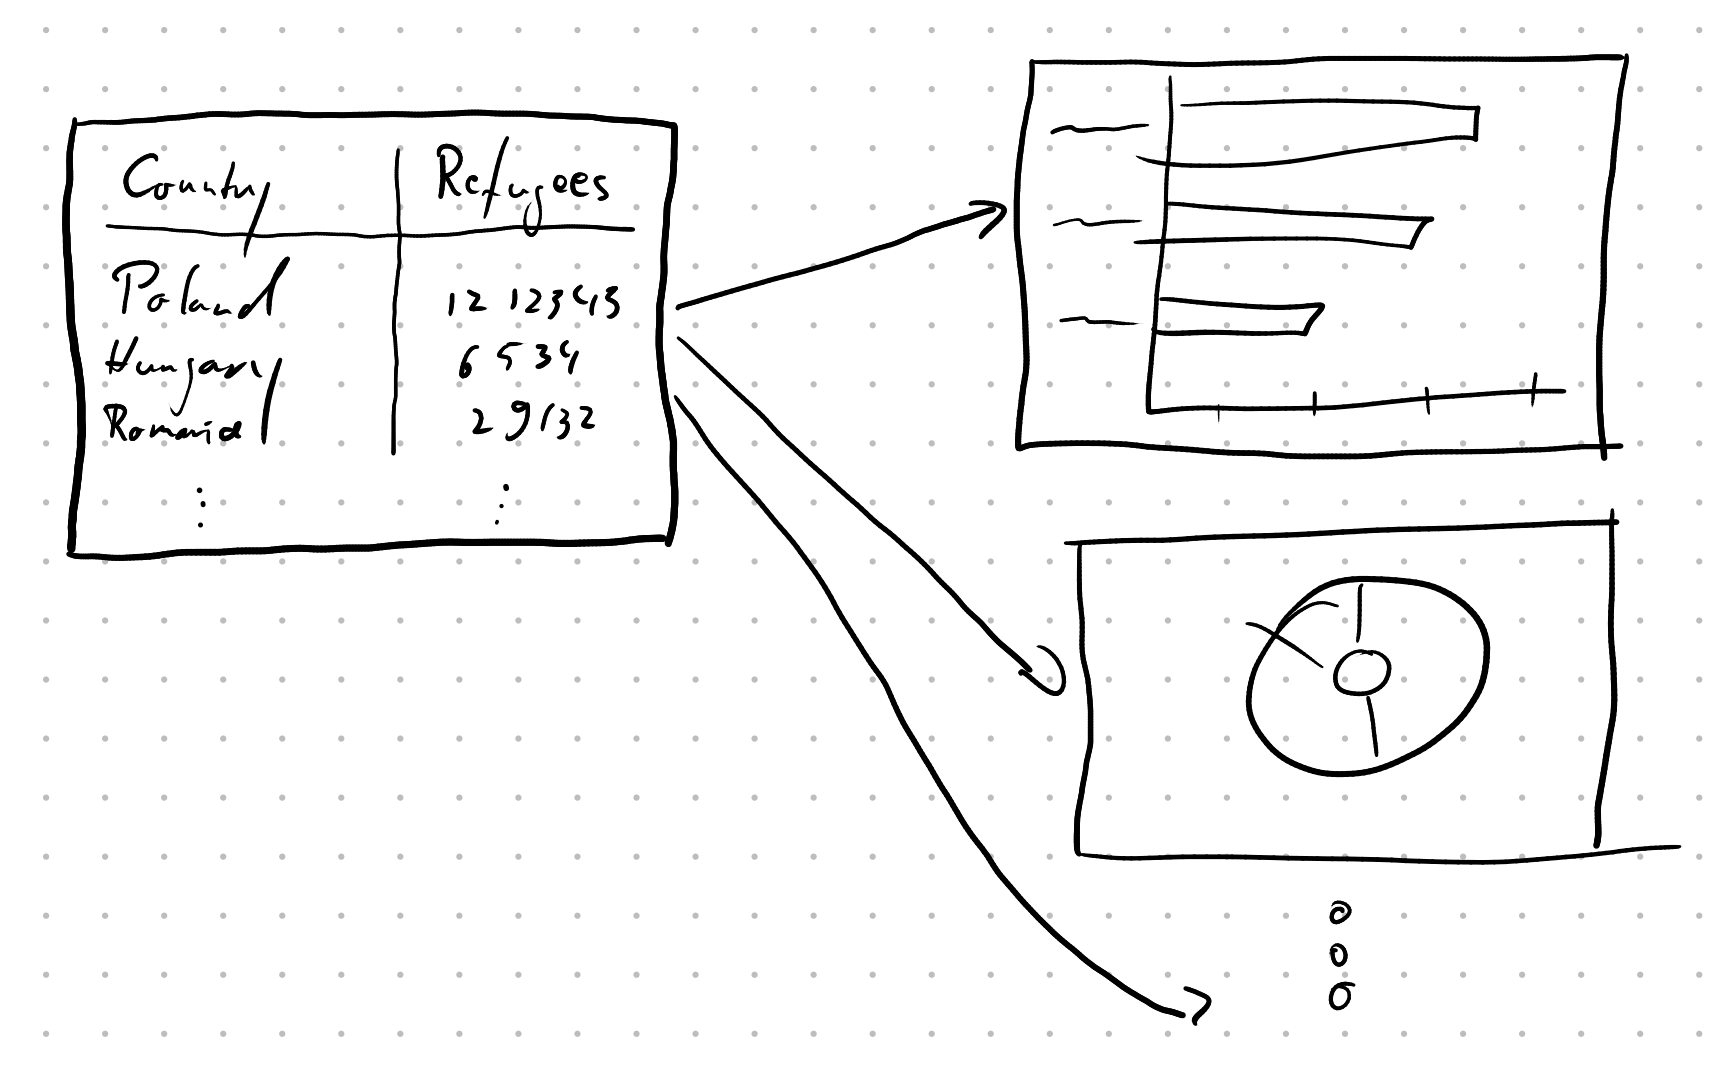
\includegraphics[width=\linewidth]{data-visualization3.png}
    \captionsetup{width=0.9\textwidth}
    \caption[data-visualization]{Data visualization describes the process of turning raw data into visual representations. There can be a multitude or possible representations for a data-set.}
    \label{fig:data-visualization}
\end{figure}

Data is commonly preprocessed before turning it into diagrams. Depending on the dataset and the desired result, this can mean different things. One might want to remove excessive information from the dataset, which is not necessary for the representation. On the other hand, additional data can be added by evaluating the existing data-points. These could for example be the median of values or grouping of certain value ranges\cite{garcia2015data}. It is important to note, that this preprocessing can happen with specific intentions in mind. While it is only supposed to make the representations easier and more concrete, it can be abused to make data align with the desired results or to create a certain emphasis. This thesis is not too concerned with this, as the possibilities of D3 are independent of the validity and completeness of the chosen data.

Even though data comes from a huge variety of sources and can express a plethora of things, there are only four different types of data\cite{henze_2021}. They are split into two categories. Categorical and numerical data. Each category has two subtypes. In the following each of the types of data will be explained.

\subsection{Categorical}
%\textcolor{red}{
%What is categorical data? Nominal and ordinal data}

Categorical or qualitative data is information collected in groups. It is often of descriptive nature. Whilst the values can be represented in numbers, they do not allow for arithmetic operations. Yet as it is possible to count the data-points, it is possible to find the mode. The mode is the most frequently occurring data.

There are two types of categorical data. Nominal and ordinal data.

\paragraph{Nominal}
data is mostly descriptive in nature. They are independent and have no inherited order. Examples are 'Country of origin', 'Color of paint', 'Brand of car'.

\paragraph{Ordinal}
data is also descriptive, yet the data does have a internal order. For example different dates each describe a day, but one day also comes after another. Grades also have an internal order, as one grade is better then another. Whilst ordinal data has an ordering, the order is not necessarily equidistant. Due to its internal order, it is also possible to find the median. The value where half the values are higher and the other half are lower.

\subsection{Numeric}
%\textcolor{red}{
%What is numeric data? Continuous and Discrete}

Numeric or quantitative data is all data expressed in numbers, where numbers do not represent categories. It allows for arithmetical operations and can be split into discrete and continuous data.

\paragraph{Discrete}
data can only take certain defined values. This usually means whole numbers to represent things that can not be split up further. Like the 'Number of Refugees' or 'Tickets sold'. Discrete data is countable.

\paragraph{Continuous}
data can be measured. It can have any real number as value. Therefore fractions are possible as well. For example when measuring the temperature, or the length or weight of an object.


\section{Diagrams}
%\textcolor{red}{
%What diagrams exists? Which are the most common? What possibilities do they offer for encoding data? Which considerations for readability? Why do some diagrams not make as much sense? Which considerations where made for fulfilling the showcase requirements?}

We constantly come across the results of data visualization in everyday life. They can be commonly found across all kinds of reports, information campaigns or as part of user-interfaces in machinery or control systems. Yet the selection of which diagram should be used to visualize which data-set is not trivial. Mostly there are several possible diagram choices for the given data. Furthermore there are a plethora of diagrams already in use and anyone can create totally new diagrams to suit their needs. Yet the vast majority of use-cases can be accomplished by one of the more commonly known diagram types, like bar and column-charts, pie and doughnut-charts, line and area-charts, scatter-plots and heat-maps. Due to their popularity, tools like Excel provide support for these diagrams out of the box\cite{office_chart_types}. More specialized diagrams might use combinations or variations of the aforementioned diagram types. 

Whilst there are countless types of diagrams, all diagrams use a combination of marks and channels to present data. Marks are used for entries in the diagram. The three possible marks are points, lines and areas. Channels describe the way specific marks encode data. The most commonly used channels are position, size, color and texture. The position in 2D can be split into the x and y positions. The color can be split into hue and luminescence. Each mark should use at least one channel to encode data. Otherwise it does not convey any information. For example in fig. \ref{fig:bar-chart} we can see lines being used as marks for each of the seven entries. It might seem like areas are used. Yet the thickness of the line, and therefore the bar, only serves visual understanding and holds no relevant information. Therefore the bar-chart, as well as column-charts, use lines as marks. The lines use three channels to encode data. The y-position is used to represent the categorical data of which country. The hue of the bar encodes the same data. This is a bit redundant, as the country is already encoded. Yet the hue makes it easy to follow along when data is changing and bars are shifting positions. The size, in this case length, of the bar encodes the discrete data of how many refugees have crossed into the country. In fig. \ref{fig:donut-chart} we see areas used as marks. Just like in the previous example the hue encodes the country and the size encodes the refugee count. 

All marks can be used with all channels. But not all data types should be represented by all channels. For example nominal data should not be encoded using the size channel. The different sizes would lead to a perceived order, which does not exist in nominal data. As the channels all differ in their appearance they are also not equally good in adequately representing the data types. Therefore it is important to consider which channels are chosen to represent the given data types. According to a study by Jock Mackinlay from 1986, the position channels can always be considered the strongest channels, no matter which marks are combined with them\cite{mackinlay1986automating}. Therefore the selection of marks and channels should be considered carefully. If chosen poorly it can lead to undermine the purpose of the diagram of easily presenting data to a viewer.
Another factor which plays a role here, is the data-ink ratio described by Edward Tufte\cite{tufte}. It describes the ratio of ink necessary for representing data over the total ink necessary for the diagram. The idea is to show only what is necessary for showing the data, as this is the main purpose of a diagram. Whilst a lot of diagrams are digital nowadays and therefore not require ink, diagrams should still try to get as close as possible to a data-ink ratio of one. The lower the data-int ratio drops, the harder it gets for a viewer to see and comprehend the relevant data.
As some viewers might not be able to perceive the whole range of colors, choosing a color scale should also be carefully considered. Besides using colors which retain a high contrast for different color blindness, they should also be perceptually uniform. Whilst most color scales have similar hues for values close together, and more distinctively different hues for values further apart, they should also be consistent in the rate of change of the hue. This is especially important when trying to encode quantitative data using the hue channel.

\begin{figure}
    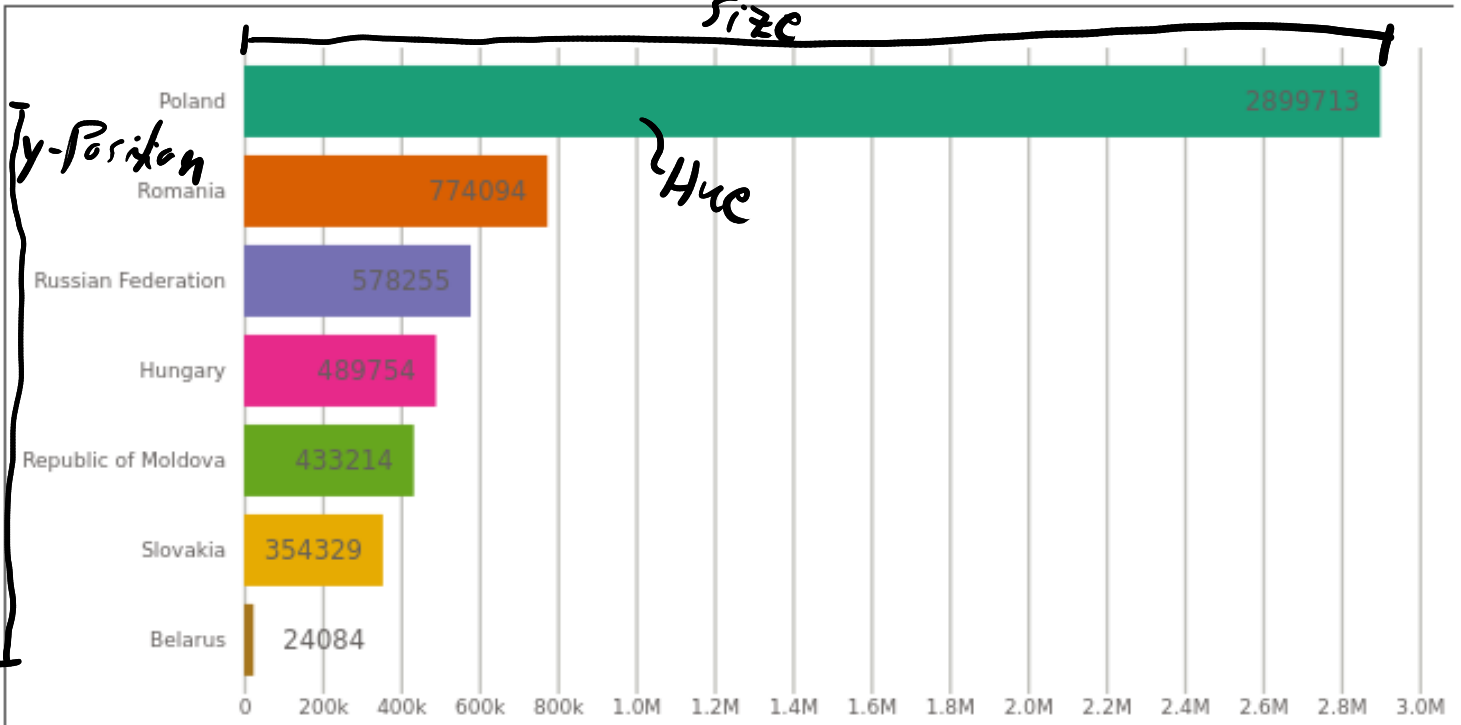
\includegraphics[width=\linewidth]{bar-chart-channels.png}
    \captionsetup{width=0.9\textwidth}
    \caption[bar-chart]{This bar-chart uses lines as marks. Each bar is a single line mark. The thickness has no relevance other than making the line visible. The three channels each mark encodes are marked. The y-position and the hue are used to encode the country. The size of the line, aka the length, corresponds to the number of refugees.}
    \label{fig:bar-chart}
\end{figure}

\begin{figure}
    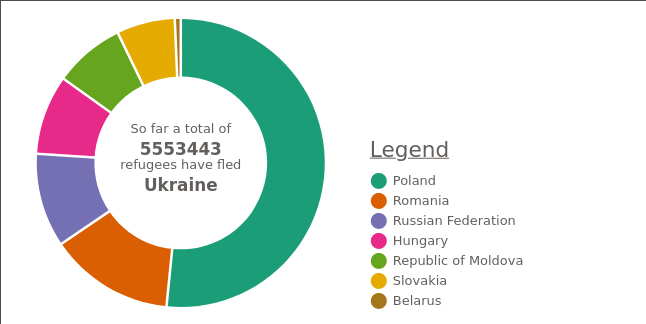
\includegraphics[width=\linewidth]{donut-chart.png}
    \captionsetup{width=0.9\textwidth}
    \caption[donut-chart]{This is a donut-chart (TODO: which needs a frame..? Also draw in marks and channels)}
    \label{fig:donut-chart}
\end{figure}

While data can already be skewed during collection and preprocessing, diagrams can do the same. Tufte introduced the lie factor for evaluating how accurately data is shown \cite{tuftevisual}. It is defined as the effect size in the diagram over the effect size in the data. Most sources of skewed representations of data can be prevented by using zero baselines, equidistant axes, accurate scaling when using areas and value adjustments for monetary values to contradict inflation influences.


\section{D3.js}
%\textcolor{red}{
%This is all about d3. What is it? Where does it come from? What is it used for? Who uses it? Why should it be used? How does it work? Enter, update and exit pattern. Something about the modular structure of D3 as well. Might be worth mentioning "observables" as well.}

While there are many ways to turn data into diagrams, this thesis makes use of D3 to achieve this. Therefore this chapter introduces D3 by elaborating what it is and how it works.

"D3.js is a JavaScript library for manipulating documents based on data. D3 helps you bring data to life using HTML, SVG, and CSS."\cite{d3js}. The name D3 is short for data-driven documents. The D3 library was originally created by Mike Bostock and is published under the BSD-3-Clause open-source license. It is about 500kb in size. It does not require a specific framework and can therefore be easily integrated into all kinds of web based projects. Whilst D3 is not limited to using svg, the visualization created using D3 mostly rely on svg elements for their implementation.

D3 is not a high-level API for creating out-of-the-box visualizations. Instead, "[it] allows you to bind arbitrary data to a Document Object Model, and then apply data-driven transformations to the document."\cite{d3js}, therefore making Document-Object-Model(DOM) manipulation easier and less tedious. The DOM represents the structure of an HTML in memory and offers scripts the possibility of accessing and modifying the represented HTML. D3 also provides helper functions like scales, to decrease the amount of mathematical equations needed to convert from the data range to the necessary coordinates in the desired visualization.

There are three main concepts that make up the core of D3. Selections, data joins and the general update pattern. All three concepts are working closely together. Whilst selections can be used without data joins and the general update pattern, these two aspects both rely on selections. Data joins can also be used without explicitly using the general update pattern. Usually all three of these concepts are used consecutively. First a selection is created. This selection is provided with a data join. Finally the behaviors for the general update pattern are defined for this data join.
In the following all three of the core concepts of D3, as well as scales and D3's packages are explained.


\subsection{Selections}
%\textcolor{red}{
%What are they? Why are they useful?}

A selection contains references to one or more DOM elements. These references are organized in groups. There are two functions in D3 to create a new selection: \verb|d3.select("selector")| and \verb|d3.selectAll("selector")|. Both functions require a selector for identifying the appropriate elements. The selectors are defined in the "W3C Selectors API"\cite{w3c_selectors_api} and function like CSS selectors. Whilst \verb|select| only selects a single element, the first element matching the selector, \verb|selectAll| selects all elements which match the selector. It is important to note, that \verb|select| also propagates the existing information of this node, whilst \verb|selectAll| does not. Selections can also be extended or shrunken by adding or removing groups, or by combining multiple selections. \verb|select| and \verb|selectAll| can also be called on on elements of an already existing selections. The selector will then assume the existing element as root for its selection process.

It is possible to directly access DOM elements through the selections. The respective DOM elements are linked in the groups which make up the selection. But usually this is not required, as there are predefined functions for easily modifying properties for all elements referenced in a selection. This includes the modification of attributes and styles of DOM-elements, as well as event handling.

A selection is required before a data-join can be made. How this is achieved is described in the following section.


\subsection{Data Joins}
%\textcolor{red}{
%What are they and why are they important?}

\begin{figure}
    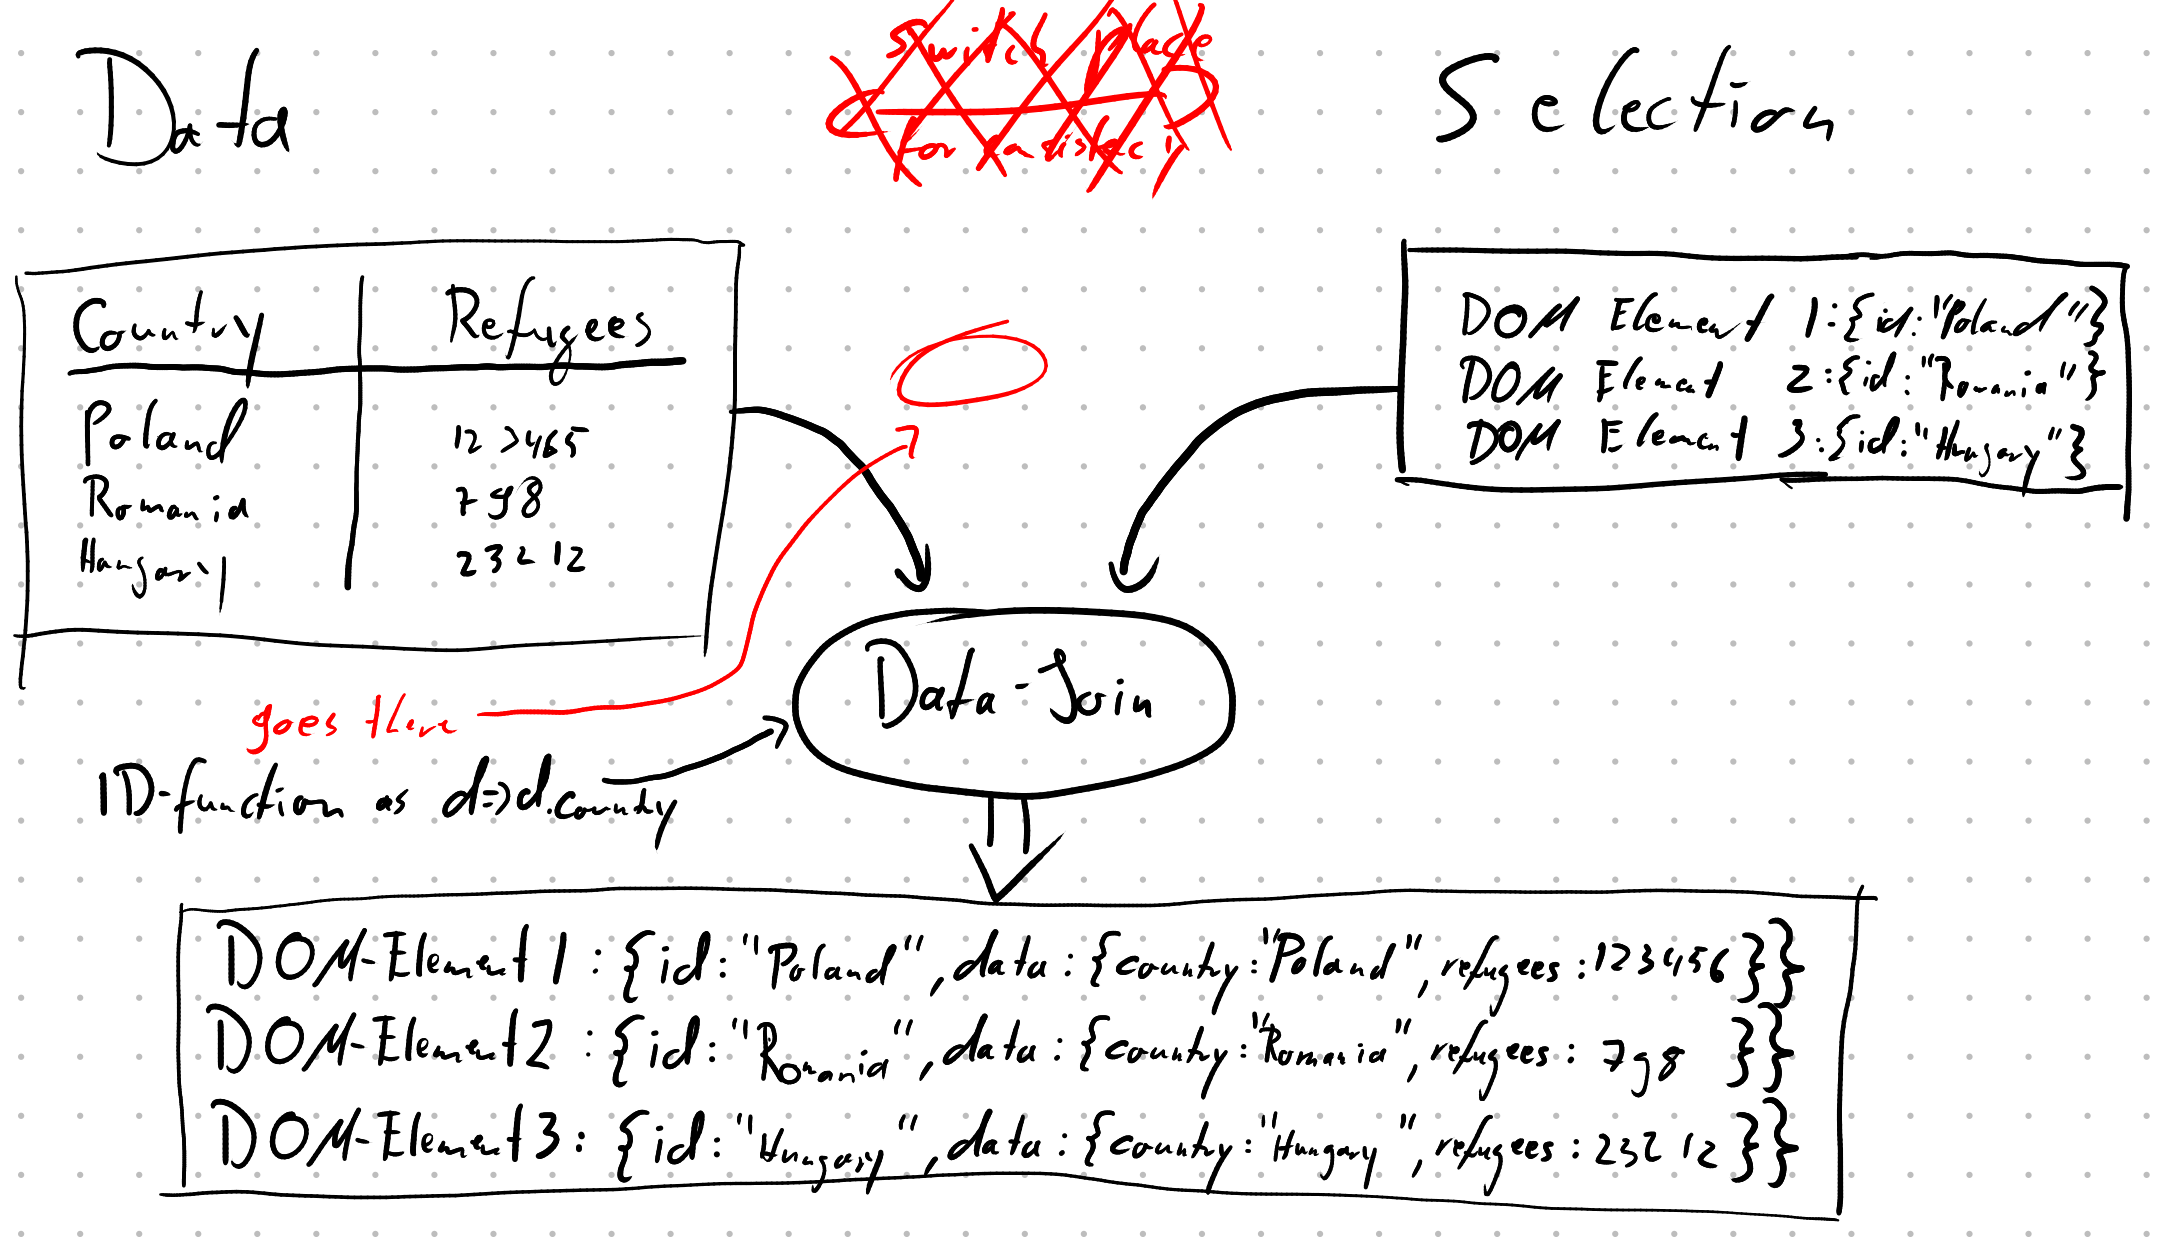
\includegraphics[width=\linewidth]{data-joins_general.png}
    \captionsetup{width=0.9\textwidth}
    \caption[data-joins]{A representation of how data-joins are created. A selection, consisting of DOM-elements, as well as the data need to be present first. The data-join then combines the two. The identifier function is needed if the diagram is supposed to be able to update and can be specified when creating the data-join. As a result the data an ID are matched to the DOM-elements.}
    \label{fig:data-joins}
\end{figure}

Data joins are the second key feature of D3. They bind a specific data-point to a specific DOM element. To create a data-join, one has to first create a selection of elements. These are the elements one wants to match to specific data points. The data join is then created by calling the \verb|.data(dataset)| function on the selection. It takes a dataset, an array of objects where each object represents a single data-point, as parameter. This will bind the data-points to the elements in the selection. This is achieved by using an identifier function. The default identifier function returns the index of the data-point in the dataset. When we want to create diagrams which can respond to data changes over time, this is not a reliable identification. When data-points are removed or added in arbitrary locations, the index will not match the elements it previously did. Therefore we can specify a custom identifier function, as seen in figure \ref{fig:data-joins}. This can be passed as the second parameter of the data function, will be called for each data-point and has to return some value which will be used as the ID. When data changes one should recreate the underlying selection, before calling the data-join again.

As seen in fig \ref{fig:general-update-pattern}, it can be that the number of data-points does not match up with the number of elements to represent them. When there is no element matched to a certain data-point, D3 will create an empty placeholder node for this data-point. What happens to the placeholders is defined in the general update pattern.


\subsection{General Update Pattern}
%\textcolor{red}{
%What is it? What can it do? Describe data joins and dom element links.}

%\begin{figure}
%    \label{fig:general-update-pattern}
%    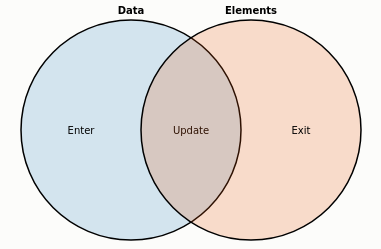
\includegraphics[width=\linewidth]{general-update-pattern.png}
%    \caption[general-update-pattern]{A visual representation of the make up of the general update pattern\cite{bostock_2012}}
%\end{figure}


\begin{figure}
    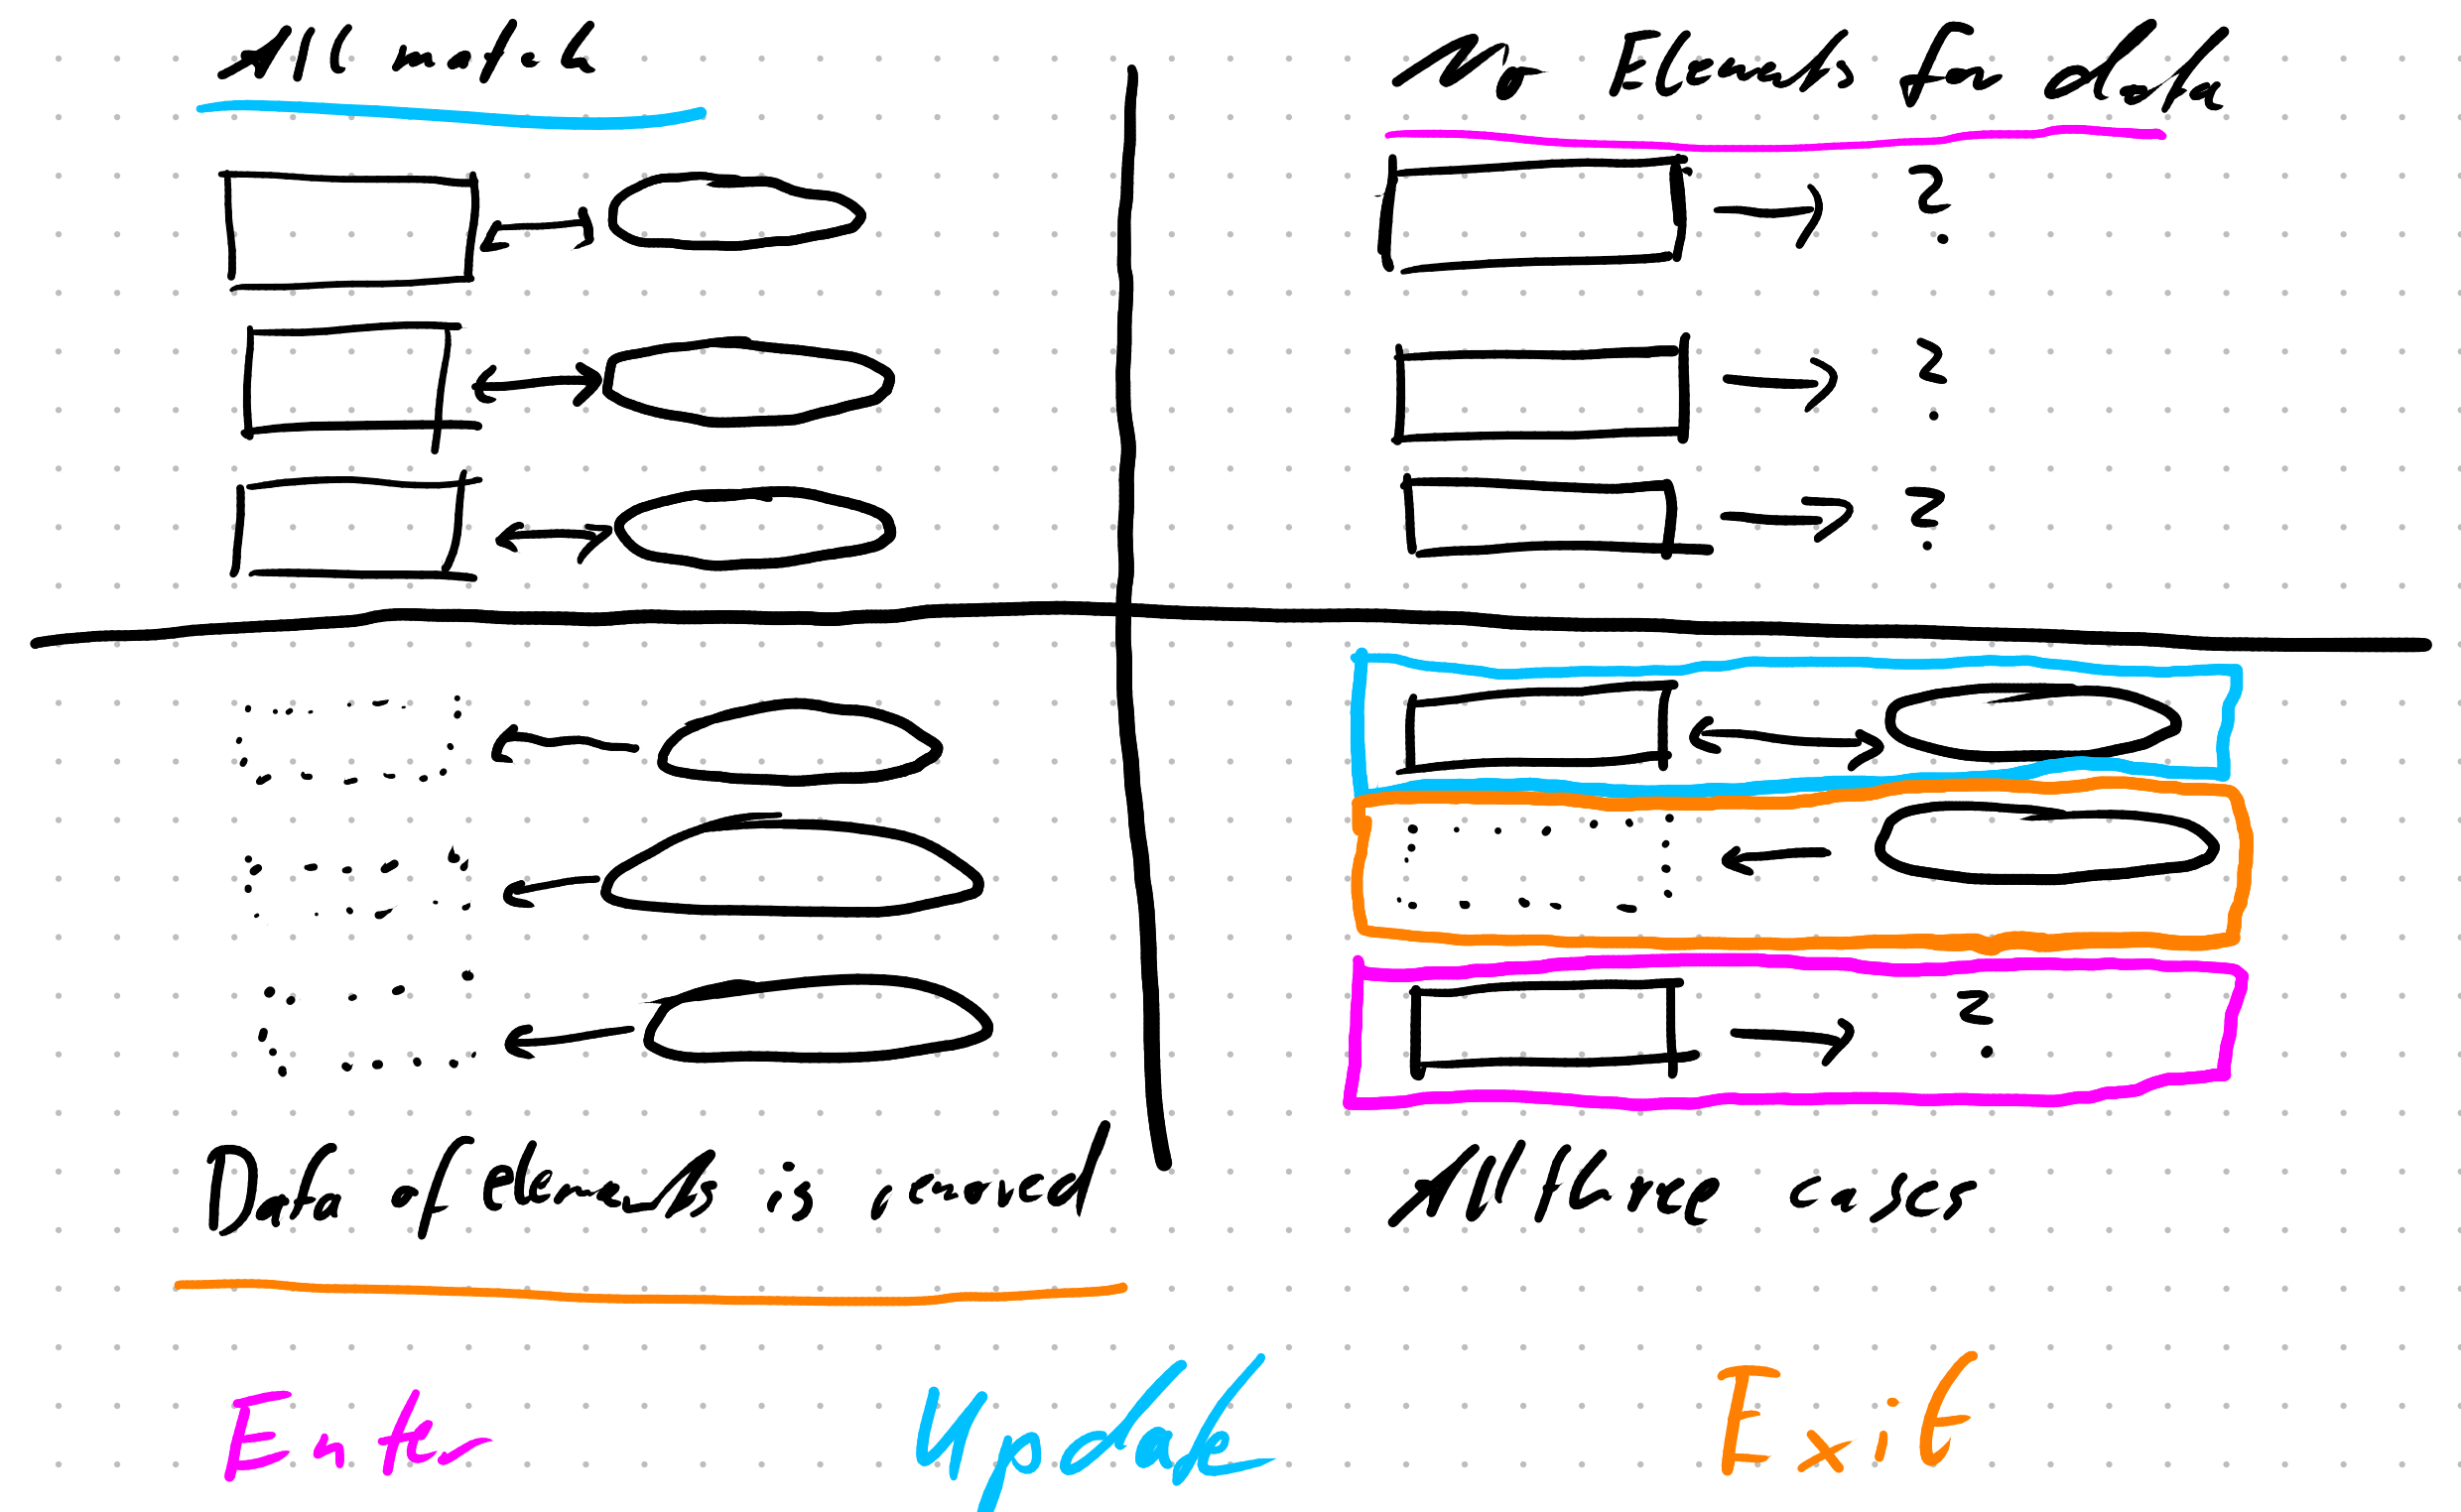
\includegraphics[width=\linewidth]{data-joins.png}
    \captionsetup{width=0.9\textwidth}
    \caption[general-update-pattern]{A representation of possible data joins. In the top left, the data join was able to match all data points to an element of the provided selection. In the top right, there are data points but no elements in the provided selection. In the bottom left, the provided selection already was filled with elements, but their corresponding data points have been removed. The bottom right shows that all three previous cases can exist in a single data-join. For each of the three resulting sub-selections, the general update pattern can have different behavior specified.}
    \label{fig:general-update-pattern}
\end{figure}

The general update pattern is another core concept of D3. Every time a data join is created or updated, it can be made use of. The general update pattern differentiates between three different cases. For each of these cases a sub-selection is created by the data-join. For each of these three sub-selections the behavior can be defined. The first selection is the enter selection. It corresponds to the pink elements in fig \ref{fig:general-update-pattern}. All the placeholders created by the data-join for data-points without a matching element are in here. In the behavior for the enter selection, usually a corresponding element is created as the first step. As each of a diagrams marks correspond to a separate element, they are created here as well. This includes providing enough attributes for the element to be appropriately matched the next time the data-join is called. Providing appropriate attributes and styles of an element which corresponds to a mark in the diagram also corresponds on using the desired channels for data encoding.

All the elements which are already linked to a data-point using the identifier function, make up the update selection. They are marked in blue in fig \ref{fig:general-update-pattern}. Specifying the behavior of the update selection allows the diagram to react to changing data by moving existing elements or changing their appearance to accommodate for other new or removed elements.

The last selection, the exit selection, is made up of all the elements for which the corresponding data-point has been removed. They are marked in orange in fig \ref{fig:general-update-pattern}. The behavior of the exit selection is by default defined to remove the respective elements.

When the goal is to create only static diagrams, which are only initially created from data, it is enough to define the behavior for the enter selection, as all data-points will be matched up with a placeholder when first creating the data-join. Here the identifier function is also not important, as the created element will not need to change over time and therefore does not need to be appropriately matched by the data-join. But if diagrams should be able to react to data changes and update their appearance, like in this thesis, it is important to define the update behavior as well as a proper identifier function, so elements are always matched with the same data-points. It is also important to provide elements which are created in the enter behavior with enough information, that the next time the data-joins underlying selection is done, the newly added elements are matched as well. The exit behavior can be defined if a more visually pleasing removal of elements is desired, like fading out before deleting.


\subsection{Scales}
%\textcolor{red}{
%What are scales? What do they do? Why and when are they used? How do they look like?}

Scales are a way to convert between two data-spaces. Some scales can even convert between two data-types. Scales can be found in many places. For example converting percentages of correct answers in a test, continuous data, to the appropriate grade, ordinal data. Or the scale factor of maps and model-kits.

As most diagrams created with D3 are created as SVG, the scales provided by D3 are, in this thesis, mostly used to convert from the data-space to the coordinate space in which elements should be drawn. All scales require a domain and a range. The domain describe the input values, the range where they should map to. Some types of scales also allow to be used in reverse. 

\subsection{Plugins}
%\textcolor{red}{
%The way D3 is split up into modules, the core package and what kind of extensions are there.}

D3 provides the most used, general functionalities in the core library. Yet there are many plugins which can be added to add functionalities for more specific use-cases. Plugins needs to be loaded additionally to the core library. This thesis makes use of the sankey plugin\cite{sankey_package}, to draw the sankey graph.

As D3 is an open-source project, the plugins available are not all created by the creator of D3, Mike Bostock. Instead a majority is created by the community using D3.
